\documentclass[tikz,border=10pt]{standalone}
\usetikzlibrary{shadings,intersections}
\begin{document}
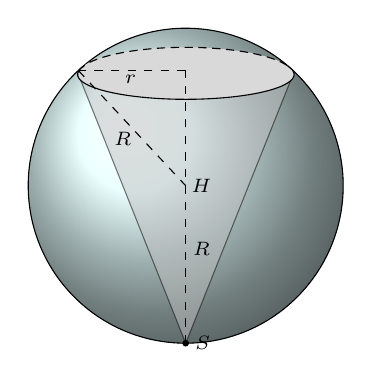
\begin{tikzpicture}
  \coordinate (O) at (0,0);

  % ball background color
  \fill[ball color=cyan!10, opacity=1.0]  (O) circle (2); % 3D lighting effect

  % cone
  \begin{scope}
    \def\rx{0.71}% horizontal radius of the ellipse
    \def\ry{0.15}% vertical radius of the ellipse
    \def\z{0.725}% distance from center of ellipse to origin

    %\path [name path = ellipse]    (0,\z) ellipse ({\rx} and {\ry});
    %\path [name path = horizontal] (-\rx,\z-\ry*\ry/\z)
                                -- (\rx,\z-\ry*\ry/\z);
    %\path [name intersections = {of = ellipse and horizontal}];

    % radius to base of cone in ball
    \draw[fill = gray!50, opacity=.5] (0,-2) -- (-1.33,1.33) -- (1.33,1.33) -- cycle;
    % base of cone in ball
    %\draw[fill = gray!30, densely dashed] (0,\z) ellipse ({\rx} and {\ry});
  \end{scope}

  % label of cone
  %\draw (0.25,0.4) -- (0.9,0.1) node at (1.05,0.0) {$q$};

  % ball
  \draw (O) circle [radius=2cm];
  % label of ball center point
  \filldraw (0,-2) circle (1pt) node[right] {\scriptsize $S$};

  % radius
  %\draw[] (0,-2) to [edge label = $R$] (-1.33,1.33);
 % \node at (-1,-0.2) {\scriptsize$R$};
 %\draw[fill = gray!30, densely dashed, opacity=0.5] (0,-2) to (1.33,1.33);

  % cut of ball surface
  %\draw[red] (-1.35,1.47) arc [start angle = 140, end angle = 40, x radius = 17.6mm, y radius = 14.75mm];
  \draw[fill = gray!30, densely dashed, opacity=1] (-1.36,1.46) arc [start angle = 170, end angle = 10, x radius = 13.8mm, y radius = 3.6mm];
  \draw[fill = gray!30, opacity=1] (-1.29,1.52) arc [start angle=-200, end angle = 20, x radius = 13.75mm, y radius = 3.15mm];

  % label of cut of ball surface
  %\draw (-1.2,2.2) -- (-0.53,1.83) node at (-1.37,2.37) {$A$};
  \draw[dashed] (0,-2) -- (0,1.46);
  \node at (0.2,0) {\scriptsize$H$};
  \draw[dashed] (0,1.46) -- (-1.36,1.46,0);
  \node at (-0.7,1.35,0) {\scriptsize$r$};
  \draw[dashed] (-1.36,1.46,0) -- (0,0);
  \node at (0.2,-0.8) {\scriptsize$R$};
  \node at (-0.8,0.6) {\scriptsize$R$};
\end{tikzpicture}
\end{document}